\chapter{音響エネルギ分布特性}
観測高さごとの音響エネルギ分布をみるため、解析で得られたインパルス応答からStrength$G$、話声に対応する明瞭度$D_{50}$、音楽に対応する明瞭度である初期/後期反射音エネルギ比$C_{80}$、初期残響時間$EDT$、初期側方反射エネルギ率$LF$、両耳間相互相関度$IACC$を算出した。
(A)矩形モデルにおける各種音響物理指標の平面コンター図、度数分布表、各指標値と音源-観測点間距離$r$[m]の関係を以下に示す。
なお、音源はコンター図内(x,y,z)=(0.0,8.0,2.5)に位置し、ステージ先端はy=10.0にあたる(\figref{zahyo})。度数分布表内の破線は各観測高さ内にある105の観測点の平均値$\mu$を表す。

\begin{figure}[htbp]
    \centering
    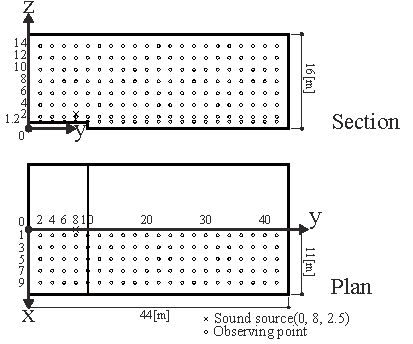
\includegraphics[keepaspectratio,scale=1]{04_att/zahyo.pdf}
    \caption{\hspace{1mm}Rectangular coordinate system of model}
    \label{fig:zahyo}
\end{figure}

\newpage
      \begin{minipage}{1\textwidth}
        \centering
          \includegraphics[keepaspectratio,width=1\hsize,angle=0]
                          {04_att/Onkyo_rec1.pdf}
      \end{minipage}
\newpage
      \begin{minipage}{1\textwidth}
        \centering
          \includegraphics[keepaspectratio,width=1\hsize,angle=0]
                          {04_att/Onkyo_rec2.pdf}
      \end{minipage}
\newpage
      \begin{minipage}{1\hsize}
        \centering
          \includegraphics[keepaspectratio,width=1\hsize,angle=0]
                          {04_att/Onkyo_rec3.pdf}
      \end{minipage}
\newpage
      \begin{minipage}{1\hsize}
        \centering
          \includegraphics[keepaspectratio,width=1\hsize,angle=0]
                          {04_att/Onkyo_rec4.pdf}
      \end{minipage}
\newpage
      \begin{minipage}{1\hsize}
        \centering
          \includegraphics[keepaspectratio,width=1\hsize,angle=0]
                          {04_att/Onkyo_rec5.pdf}
      \end{minipage}
\newpage
      \begin{minipage}{1\hsize}
        \centering
          \includegraphics[keepaspectratio,width=1\hsize,angle=0]
                          {04_att/Onkyo_rec6.pdf}
      \end{minipage}      
\newpage
      \begin{minipage}{1\hsize}
        \centering
          \includegraphics[keepaspectratio,width=1\hsize,angle=0]
                          {04_att/Onkyo_rec7.pdf}
      \end{minipage}      

一元配置分散分析(対応あり)の結果を\tabref{ichigen}に示す。
$EDT$を除く全ての指標値で有意な差が認められた。
次にHolmの多重比較を行った結果を\tabref{Gtaju}$\sim$\tabref{Ttaju}に示す。


\begin{table}[H]
\centering
\caption{The result of one-way analysis of variance}
\label{tab:ichigen}
\begin{tabular}{cccccccc}
\Hline
\begin{tabular}[c]{@{}c@{}}Acoustic\\ parameter\end{tabular} & \textit{G} & \textit{EDT} & $C_{80}$ & $D_{50}$ & \textit{LF} & \textit{IACC} & $T_{30}$ \\ \hline
judge & ** & n.s. & * & ** & ** & ** & ** \\ \Hline
\multicolumn{8}{l}{**:$p$\textless{}0.01, *:$p$\textless{}0.05}
\end{tabular}
\end{table}

\begin{table}[H]
\centering
\caption{$G$ of the test results}
\label{tab:Gtaju}
\begin{tabular}{ccccccccc}
\Hline
 & 1.2 & 2.0 & 4.0 & 6.0 & 8.0 & 10.0 & 12.0 & 14.0 \\ \hline
1.2 &  & n.s. & n.s. & n.s. & n.s. & n.s. & n.s. & n.s. \\
2.0 &  &  & n.s. & n.s. & n.s. & n.s. & * & ** \\
4.0 &  &  &  & n.s. & n.s. & n.s. & ** & ** \\
6.0 &  &  &  &  & n.s. & n.s. & n.s. & n.s. \\
8.0 &  &  &  &  &  & n.s. & n.s. & n.s. \\
10.0 &  &  &  &  &  &  & n.s. & n.s. \\
12.0 &  &  &  &  &  &  &  & n.s. \\
14.0 &  &  &  &  &  &  &  &  \\ \Hline
\end{tabular}
\end{table}

\begin{table}[H]
\centering
\caption{$D_{50}$ of the test results}
\label{tab:Dtaju}
\begin{tabular}{ccccccccc}
\Hline
 & 1.2 & 2.0 & 4.0 & 6.0 & 8.0 & 10.0 & 12.0 & 14.0 \\ \hline
1.2 &  & n.s. & n.s. & n.s. & n.s. & n.s. & n.s. & n.s. \\
2.0 &  &  & n.s. & n.s. & n.s. & n.s. & n.s. & n.s. \\
4.0 &  &  &  & n.s. & n.s. & n.s. & n.s. & n.s. \\
6.0 &  &  &  &  & n.s. & n.s. & n.s. & n.s. \\
8.0 &  &  &  &  &  & n.s. & n.s. & * \\
10.0 &  &  &  &  &  &  & n.s. & * \\
12.0 &  &  &  &  &  &  &  & n.s. \\
14.0 &  &  &  &  &  &  &  &  \\ \Hline
\end{tabular}
\end{table}

\begin{table}[H]
\centering
\caption{$LF$ of the test results}
\label{tab:LFtaju}
\begin{tabular}{ccccccccc}
\Hline
 & 1.2 & 2.0 & 4.0 & 6.0 & 8.0 & 10.0 & 12.0 & 14.0 \\ \hline
1.2 &  & n.s. & n.s. & n.s. & * & ** & ** & ** \\
2.0 &  &  & n.s. & n.s. & * & ** & ** & ** \\
4.0 &  &  &  & n.s. & * & ** & ** & ** \\
6.0 &  &  &  &  & n.s. & * & ** & ** \\
8.0 &  &  &  &  &  & n.s. & * & ** \\
10.0 &  &  &  &  &  &  & n.s. & n.s. \\
12.0 &  &  &  &  &  &  &  & n.s. \\
14.0 &  &  &  &  &  &  &  &  \\ \Hline
\end{tabular}
\end{table}

\begin{table}[H]
\centering
\caption{$IACC$ of the test results}
\label{tab:IACCtaju}
\begin{tabular}{ccccccccc}
\Hline
 & 1.2 & 2.0 & 4.0 & 6.0 & 8.0 & 10.0 & 12.0 & 14.0 \\ \hline
1.2 &  & n.s. & n.s. & n.s. & n.s. & ** & ** & ** \\
2.0 &  &  & n.s. & n.s. & n.s. & n.s. & ** & ** \\
4.0 &  &  &  & n.s. & n.s. & n.s. & ** & ** \\
6.0 &  &  &  &  & n.s. & n.s. & ** & ** \\
8.0 &  &  &  &  &  & n.s. & * & ** \\
10.0 &  &  &  &  &  &  & n.s. & ** \\
12.0 &  &  &  &  &  &  &  & n.s. \\
14.0 &  &  &  &  &  &  &  &  \\ \Hline
\end{tabular}
\end{table}

\begin{table}[H]
\centering
\caption{$T_{30}$ of the test results}
\label{tab:Ttaju}
\begin{tabular}{ccccccccc}
\Hline
 & 1.2 & 2.0 & 4.0 & 6.0 & 8.0 & 10.0 & 12.0 & 14.0 \\ \hline
1.2 &  & ** & n.s. & ** & ** & ** & ** & ** \\
2.0 &  &  & n.s. & ** & ** & ** & ** & ** \\
4.0 &  &  &  & ** & ** & ** & ** & ** \\
6.0 &  &  &  &  & ** & n.s. & n.s. & n.s. \\
8.0 &  &  &  &  &  & n.s. & n.s. & ** \\
10.0 &  &  &  &  &  &  & n.s. & * \\
12.0 &  &  &  &  &  &  &  & * \\
14.0 &  &  &  &  &  &  &  &  \\ \Hline
\end{tabular}
\end{table}

残響エネルギ特性に関する指標$T_{30}$や反射音の方向情報より算出される指標$LF,IACC$では観測高さによる平均値の違いが多く見られた一方、時間エネルギ特性に関する指標$D_{50},C_{80}$及び音圧レベル特性に関する指標$G$では、観測高さによる平均値の違いはあまりみられなかった。

ここで、$G$及び$G_{early}$,$G_{late}$,$C_{80}$と音源-観測点間距離$r$[m]の関係をBarronによる理論値と共に\figref{G_Barron},\figref{Ge_Barron},\figref{Gl_Barron},\figref{C_Barron}に示す。観測高さ$H$=14.0の観測点は音源から遠い位置に分布しているため、いずれの指標値も値が一定の範囲内に集中している。このことから、座席面遠方音場ではその観測高さ内でとる各指標値のバラつきが小さくなる様子が伺える。

\begin{figure}[htbp]
    \centering
    \includegraphics[keepaspectratio,scale=1]{04_att/G_Barron.png}
    \caption{\hspace{1mm}$G$ vs distance between sound source and observing point}
    \label{fig:G_Barron}
\end{figure}

\begin{figure}[htbp]
    \centering
    \includegraphics[keepaspectratio,scale=1]{04_att/Ge_Barron.png}
    \caption{\hspace{1mm}$G_{early}$ vs distance between sound source and observing point}
    \label{fig:Ge_Barron}
\end{figure}

\begin{figure}[htbp]
    \centering
    \includegraphics[keepaspectratio,scale=1]{04_att/Gl_Barron.png}
    \caption{\hspace{1mm}$G_{late}$ vs distance between sound source and observing point}
    \label{fig:Gl_Barron}
\end{figure}

\begin{figure}[htbp]
    \centering
    \includegraphics[keepaspectratio,scale=1]{04_att/C_Barron.png}
    \caption{\hspace{1mm}$C_{80}$ vs distance between sound source and observing point}
    \label{fig:C_Barron}
\end{figure}

そこで、音響エネルギ分布の一様度をみるため、各指標それぞれの平均値と標準偏差を観測高さごとに求めた(\figref{G},\figref{Ge},\figref{Gl},\figref{C})。
\\ まず$G$を見てみる。平均値の観測高さによる変化幅は0.4dB(6.6$\sim$7.0dB)とほぼ一定の値を示した一方、標準偏差の観測高さによる変化幅は1.3dB(3.1$\sim$1.8dB)であった。これは$G$の弁別閾($\geq$1dB)を上回るため、有意な差であるといえる。加えて、観測高さが上がるにつれて標準偏差が小さくなる傾向が確認できる。
\\ 次に$G_{early}$を見てみる。平均値の変化幅は0.4dB(3.4$\sim$3.8dB)と大きな変動は見られない。一方、標準偏差の変化幅は2.0dB(2.3$\sim$4.2dB)であり、有意な差が確認できた。$G_{early}$は初期音(直接音+初期反射音)から算出される指標であるため、観測点位置による音響エネルギ分布の違いが顕著であったと考えられる。
\\ $G_{late}$をみてみる。平均値の変化幅は0.2dB(1.4$\sim$1.6dB)とほぼ一定の値であった。また、標準偏差の変化幅についても0.2dB(3.7$\sim$3.9dB)とおおよそ一定の値であった。これらより、後期音においては観測高さによる音響エネルギ分布の違いは小さいと考えられる。後期音はその空間内においてが十分に拡散した状態であるから観測点位置による違いが出にくかったものと推察できる。
\\ 最後に$C_{80}$についてみてみる。平均値の変化幅は0.4dB(-0.4$\sim$0.0dB)とほぼ一定の値をとるが、標準偏差の変化幅は1.8dB(1.0$\sim$2.8dB)であった。これは、$C_{80}$の弁別域($\geq$1dB)を上回るため、有意な差である。また、$G$と同様に$C_{80}$も観測高さが上がるにつれて標準偏差が小さくなる傾向が見られた。
\\ 以上の分析から、座席面遠方音場では近傍音場に比べ音響エネルギ分布がより一様であることがわかる。
